\chapter{Monte-Carlo et réduction de variance (call européen)}

Ce chapitre réunit la méthode de Monte-Carlo \emph{de base} et son \emph{optimisation} par réduction de variance. Le call européen sert de banc d'essai : comme on connaît $\CBS = 10{,}4506$, on peut mesurer exactement l'erreur de la simulation.

\section{Principe et algorithme}

Le prix est une espérance : $C = \E[Y]$ avec $Y = e^{-rT}(S_T-K)^+$ (on garde les notations du code). Monte-Carlo la remplace par la moyenne de $N$ simulations indépendantes :
\[
\hat C = \frac1N\sum_{i=1}^N Y_i,\qquad Y_i = e^{-rT}\big(S_T^{(i)}-K\big)^+,\qquad S_T^{(i)} = S_0\exp\Big[\Big(r-\frac{\sigma^2}2\Big)T+\sigma\sqrt T\,Z_i\Big].
\]

\begin{figure}[H]
\centering
\begin{tikzpicture}[node distance=0.45cm,box/.style={draw=bleu,rounded corners,fill=gris,text width=11.5cm,minimum height=0.9cm,align=left,font=\small},num/.style={circle,fill=bleu,text=white,font=\bfseries,minimum size=0.7cm}]
\node[box] (a) {Tirer $N$ valeurs $Z_i\sim\Ncal(0,1)$ par la méthode de Box-Muller (générateur fixé, graine 2026).};
\node[box,below=of a] (b) {Simuler $S_T^{(i)} = S_0\exp[(r-\sigma^2/2)T+\sigma\sqrt TZ_i]$ (formule exacte : pas d'erreur de discrétisation).};
\node[box,below=of b] (c) {Calculer le payoff actualisé $Y_i = e^{-rT}\max(S_T^{(i)}-K,0)$.};
\node[box,below=of c] (d) {Estimer le prix $\hat C = \frac1N\sum Y_i$ et l'IC à 95 \% : $\hat C\pm1{,}96\,s/\sqrt N$.};
\foreach \n/\k in {a/1,b/2,c/3,d/4} \node[num,left=0.3cm of \n] {\k};
\end{tikzpicture}
\caption{Algorithme de Monte-Carlo en quatre étapes (méthode de base).}
\end{figure}

\section{Étape 1 : générateur fixé et méthode de Box-Muller}\label{sec:bm}

\paragraph{Le générateur est fixé.} Le générateur de NumPy produit des nombres \emph{uniformes} sur $[0,1[$ à partir d'une \emph{graine}. Avec la même graine, on obtient exactement la même suite de nombres : les résultats de ce rapport sont reproductibles à l'identique. Dans le code : \texttt{rng = np.random.default\_rng(2026)}, un seul générateur créé au début et utilisé par toutes les fonctions ; en exécutant le notebook du début à la fin, on retrouve exactement les mêmes chiffres.

\paragraph{La méthode de Box-Muller.} L'algorithme a besoin de tirages $Z\sim\Ncal(0,1)$, alors que le générateur ne donne que des uniformes. Nous les fabriquons avec la formule de Box-Muller :
\[
\boxed{Z = \sqrt{-2\ln U_1}\,\cos(2\pi U_2)},\qquad U_1,U_2 \text{ indépendantes, uniformes sur } ]0,1].
\]
Chaque $Z$ utilise deux uniformes ; nous ne gardons qu'\textbf{une seule} gaussienne par couple $(U_1,U_2)$.

\begin{demo}[ — la formule de Box-Muller donne une loi $\Ncal(0,1)$]
On pose $R = \sqrt{-2\ln U_1}$ et $\Theta = 2\pi U_2$.

\textbf{1. Loi de $\Theta$.} $\Theta$ est uniforme sur $[0,2\pi[$, de densité $\frac{1}{2\pi}$.

\textbf{2. Loi de $R$.} Pour $t\ge0$ : $\ \Q(R^2>t) = \Q(-2\ln U_1>t) = \Q(U_1<e^{-t/2}) = e^{-t/2}$. Donc $\Q(R\le r) = 1-e^{-r^2/2}$ et, en dérivant, $f_R(r) = r\,e^{-r^2/2}$ pour $r>0$.

\textbf{3. Loi du couple.} $U_1$ et $U_2$ étant indépendantes, $R$ et $\Theta$ le sont aussi : $f_{R,\Theta}(r,\theta) = \frac{1}{2\pi}\,r\,e^{-r^2/2}$.

\textbf{4. Changement de variables.} Avec $x = r\cos\theta$, $y = r\sin\theta$, on a $dx\,dy = r\,dr\,d\theta$ et $r^2 = x^2+y^2$ :
\[
f(x,y) = \frac{1}{2\pi}e^{-(x^2+y^2)/2} = \frac{e^{-x^2/2}}{\sqrt{2\pi}}\times\frac{e^{-y^2/2}}{\sqrt{2\pi}}.
\]
\textbf{5. Conclusion.} La densité de $x = R\cos\Theta$ est $\frac{1}{\sqrt{2\pi}}e^{-x^2/2}$ : $Z = R\cos\Theta$ suit la loi $\Ncal(0,1)$.
\end{demo}

\textbf{Détail pratique.} Le générateur renvoie $U\in[0,1[$, qui peut valoir 0. On prend $U_1 = 1-U\in\,]0,1]$ pour ne jamais calculer $\ln 0$.

\textbf{Exemple à la main.} $U_1 = 0{,}5$, $U_2 = 0{,}125$ : $Z = \sqrt{-2\ln0{,}5}\times\cos(\pi/4) = 1{,}1774\times0{,}7071 = 0{,}8326$.

\textbf{Vérification sur un million de tirages.} Moyenne $-0{,}0010$ (théorie 0), variance $0{,}9987$ (théorie 1), $\Q(|Z|\le1{,}96) = 0{,}9503$ (théorie 0,95). L'histogramme suit la densité de $\Ncal(0,1)$ (figure~\ref{fig:bm}).

\begin{figure}[H]
\centering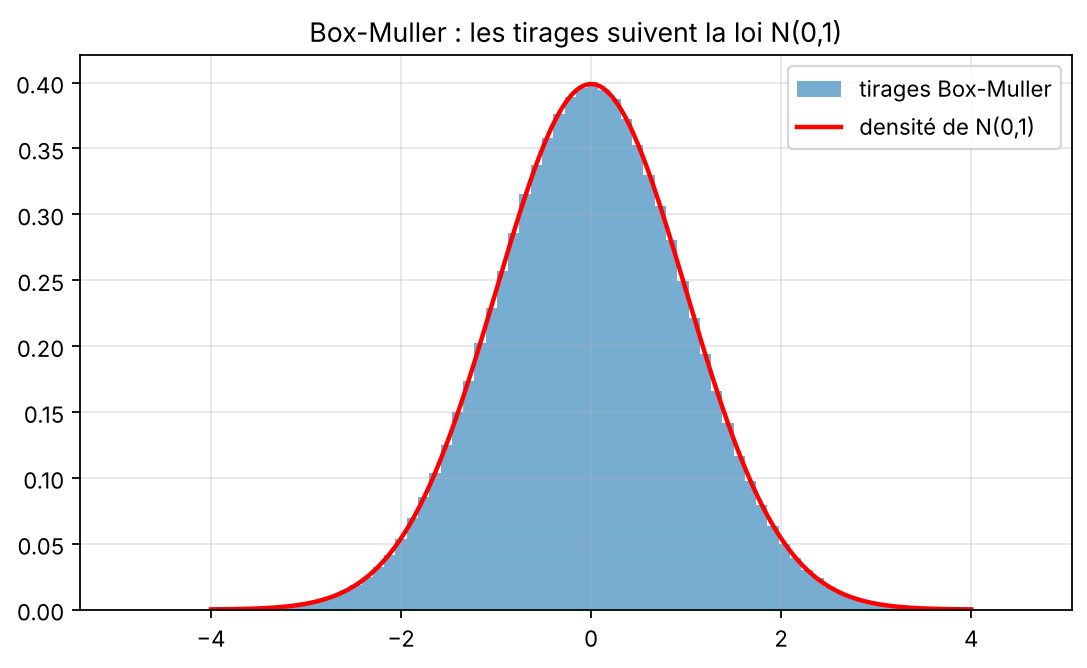
\includegraphics[width=0.7\textwidth]{fig_box_muller}
\caption{Un million de tirages de Box-Muller et la densité de la loi $\Ncal(0,1)$.}
\label{fig:bm}
\end{figure}

\section{Propriétés de l'estimateur}

\begin{demo}[ — sans biais, convergence, intervalle de confiance]
\textbf{Sans biais.} $\E[\hat C] = \frac1N\sum_i\E[Y_i] = C$.

\textbf{Convergence.} Les $Y_i$ sont indépendants et de même loi ; par la loi des grands nombres, $\hat C\to C$ quand $N\to\infty$.

\textbf{Variance.} Par indépendance, $\Var(\hat C) = \frac{\sigma_Y^2}{N}$ : l'erreur typique vaut $\sigma_Y/\sqrt N$.

\textbf{Intervalle de confiance.} Par le théorème central limite, $\sqrt N(\hat C-C)/\sigma_Y$ suit approximativement la loi $\Ncal(0,1)$. Comme $\Q(|\Ncal(0,1)|\le1{,}96) = 0{,}95$, et en remplaçant $\sigma_Y$ inconnu par l'écart-type empirique $s$ (calculé avec $N-1$ au dénominateur) :
\[
IC_{95\%} = \Big[\hat C - 1{,}96\frac{s}{\sqrt N}\ ;\ \hat C + 1{,}96\frac{s}{\sqrt N}\Big].
\]
\end{demo}

\begin{retenir}
La demi-largeur de l'IC décroît en $1/\sqrt N$ : pour diviser l'erreur par 10, il faut \textbf{100 fois plus} de simulations. Pour réduire l'erreur $1{,}96\,\sigma_Y/\sqrt N$, on peut augmenter $N$ (coûteux) ou diminuer $\sigma_Y$ : c'est la réduction de variance (section~\ref{sec:rv}).
\end{retenir}

\section{Résultats du Monte-Carlo standard}

On note $SE = s/\sqrt N$ l'\textbf{erreur standard} (l'écart-type de l'estimateur) ; l'IC à 95 \% est $\hat C\pm1{,}96\,SE$.

\textbf{Exemple à la main.} $Z = +1$ donne $S_T = 100\,e^{0{,}03+0{,}2} = 125{,}86$ et un payoff actualisé de $25{,}86\,e^{-0{,}05} = 24{,}60$. $Z = -1$ donne $S_T = 84{,}37<K$ et un payoff nul.

\textbf{Avec $N = 10^6$ simulations :}
\[
\hat C_{MC} = 10{,}4370,\qquad SE = 0{,}01471,\qquad IC_{95\%} = [10{,}4081\ ;\ 10{,}4658],\qquad \CBS = 10{,}4506\in IC.
\]
\textbf{Erreur par rapport au prix analytique :} $|\CBS - \hat C_{MC}| = 0{,}013624$.

\begin{figure}[H]
\centering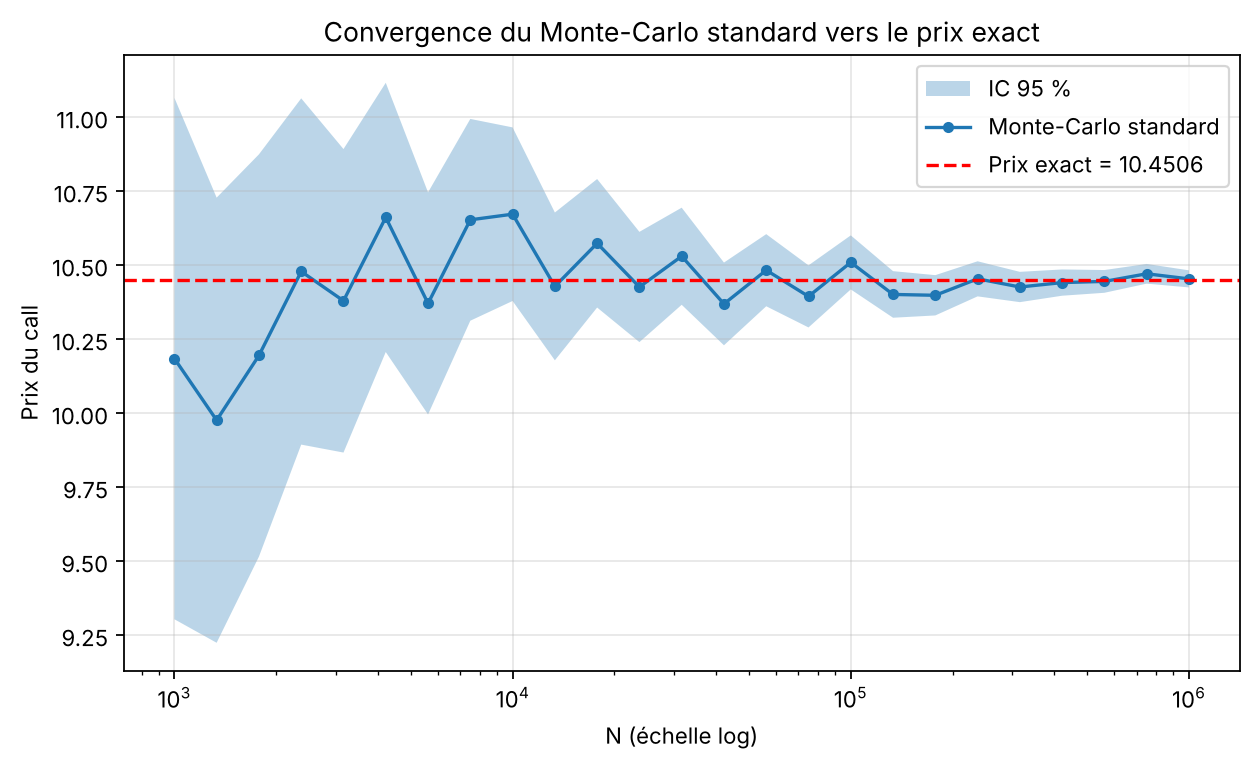
\includegraphics[width=0.82\textwidth]{fig_ic_vs_N}
\caption{Prix Monte-Carlo et IC à 95 \% pour 25 valeurs de $N$ entre $10^3$ et $10^6$.}
\label{fig:icN}
\end{figure}

\textbf{Lecture.} Quand $N$ augmente, l'intervalle se resserre autour de $10{,}4506$ : c'est la convergence de Monte-Carlo. Pour les 25 valeurs de $N$, le prix exact est dans l'IC. La largeur suit la loi $1/\sqrt N$ : multiplier $N$ par 1\,000 divise l'IC par environ $\sqrt{1000}\approx31{,}6$.

\subsection*{Prix pour les puissances de 10}
\begin{table}[H]
\centering\small
\begin{tabular}{rccc}
\toprule
$N$ & Prix MC & IC à 95 \% & Erreur $|\CBS - \hat C|$ \\
\midrule
10 & 11,9906 & [3,8810 ; 20,1002] & 1,5400 \\
100 & 10,1197 & [7,1120 ; 13,1275] & 0,3309 \\
1\,000 & 10,4897 & [9,5733 ; 11,4061] & 0,0391 \\
10\,000 & 10,5740 & [10,2834 ; 10,8645] & 0,1234 \\
100\,000 & 10,4234 & [10,3326 ; 10,5141] & 0,0272 \\
1\,000\,000 & 10,4371 & [10,4083 ; 10,4660] & 0,0134 \\
\bottomrule
\end{tabular}
\caption{Monte-Carlo standard pour $N = 10^1, \dots, 10^6$.}
\end{table}
À chaque puissance de 10, l'IC est divisé par environ $\sqrt{10}\approx3{,}16$ et contient toujours $\CBS$. L'erreur d'une seule simulation dépend du hasard (elle est plus grande à $10^4$ qu'à $10^3$) ; c'est la largeur de l'IC qui diminue toujours.

\subsection*{Trajectoire de l'estimateur : stabilité}
On suit la moyenne des $n$ premiers payoffs, $\hat C_n = \frac1n\sum_{i\le n}Y_i$, pour $n$ de 1 à $10^6$ (une seule simulation).
\begin{figure}[H]
\centering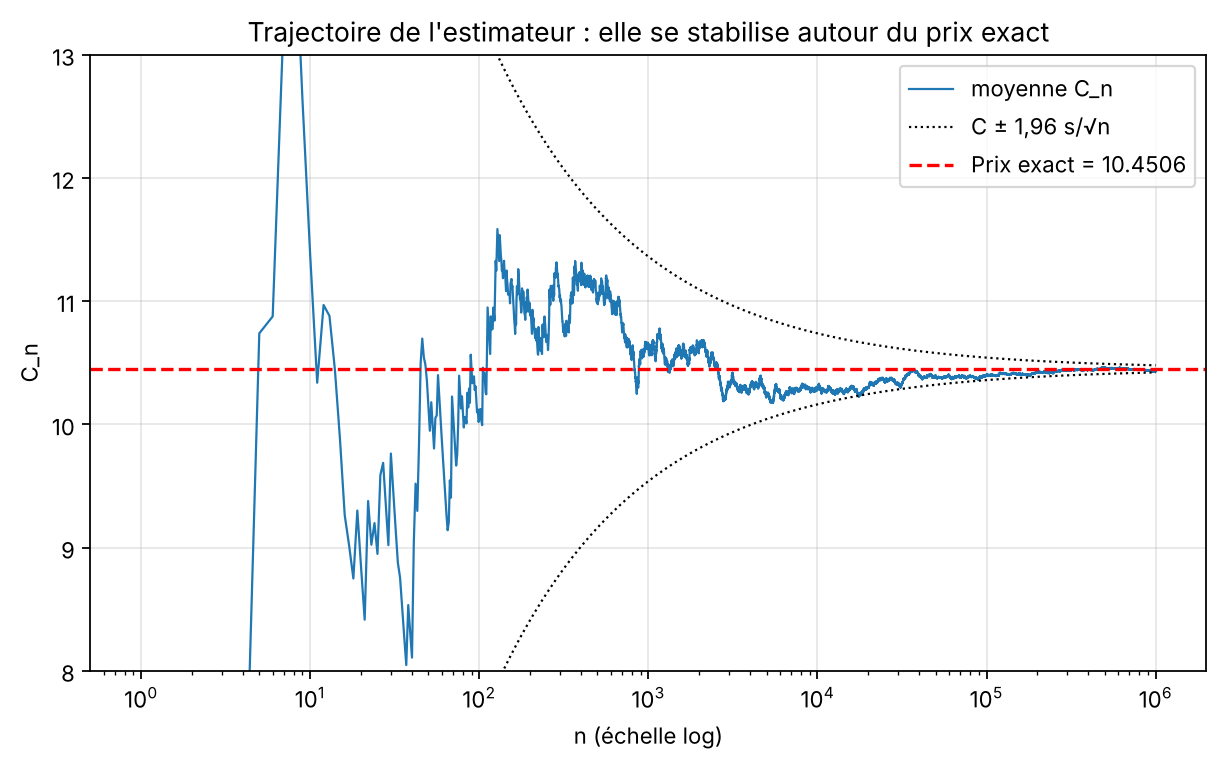
\includegraphics[width=0.82\textwidth]{fig_trajectoire}
\caption{Trajectoire $\hat C_n$ et enveloppe $\CBS\pm1{,}96\,s/\sqrt n$.}
\label{fig:traj}
\end{figure}
La moyenne bouge beaucoup au début ($\hat C_{1000} = 10{,}6402$), puis se stabilise dans l'enveloppe ($\hat C_{10^6} = 10{,}4308$) : c'est la loi des grands nombres.

\section{Réduction de variance}\label{sec:rv}

On remplace $Y$ par une autre variable \textbf{de même espérance} $C$ mais \textbf{de plus petite variance}. Toutes les méthodes sont comparées \emph{à budget égal} : $N$ payoffs chacune.

\subsection{Méthode 1 : les variables antithétiques}

Pour chaque tirage $Z$, on utilise aussi $-Z$, qui a exactement la même loi. On tire $N/2$ valeurs $Z_i$ (donc $N$ payoffs au total) et on pose $Y^+ = Y(Z)$, $Y^- = Y(-Z)$ :
\[
\hat C_{a} = \frac{1}{N/2}\sum_{i=1}^{N/2}\frac{Y^+_i+Y^-_i}{2}.
\]

\begin{demo}[ — biais et variance de l'estimateur antithétique]
\textbf{Sans biais.} $-Z$ a la même loi que $Z$, donc $\E[Y^-] = \E[Y^+] = C$ et $\E[\hat C_a] = C$.

\textbf{Variance.} Avec $\rho = \Corr(Y^+,Y^-)$ :
\[
\Var\Big(\frac{Y^++Y^-}{2}\Big) = \frac14\big(\sigma_Y^2+\sigma_Y^2+2\rho\sigma_Y^2\big) = \frac{\sigma_Y^2}{2}(1+\rho).
\]
Avec $N/2$ paires indépendantes : $\Var(\hat C_a) = \frac{\sigma_Y^2(1+\rho)}{N}$, donc
\[
\boxed{\text{gain}_{a} = \frac{\Var(\hat C_{MC})}{\Var(\hat C_a)} = \frac{1}{1+\rho}}.
\]
\textbf{Quand ça marche.} Il faut $\rho<0$. Le payoff du call augmente avec $Z$ : quand $Y^+$ est grand, $Y^-$ est petit, donc $\rho<0$.
\end{demo}

\textbf{Résultat ($N = 10^6$).} $\hat C_a = 10{,}4600$, $SE = 0{,}01039$ contre $0{,}01471$ en standard : gain de variance $(0{,}01471/0{,}01039)^2 = 2{,}00$, ce qui correspond à $\rho\approx-0{,}50$. Erreur par rapport au prix analytique : $|\CBS - \hat C_a| = 0{,}009445$.

\textbf{Pourquoi le gain n'est que de 2.} Le payoff du call est \emph{convexe} : il est nul quand $Z$ est négatif, puis croît comme une exponentielle. Quand $Z$ est grand, $Y^+$ est grand et $Y^- = 0$ : la paire ne se compense pas. La corrélation n'est que de $-0{,}5$, d'où un gain de 2.

\subsection{Méthode 2 : la variable de contrôle et le calcul de $c$}

On utilise une variable $X$ \textbf{corrélée} au payoff $Y$ dont on connaît \textbf{exactement} l'espérance : $X = S_T$, avec $\E[S_T] = S_0e^{rT}$ (chapitre 2). Pour un réel $c$ :
\[
Y_c = Y - c\,\big(X-\E[X]\big).
\]
\textbf{Idée.} Quand $S_T$ dépasse sa moyenne, le payoff est probablement grand aussi : on retire cet excès « prévisible ». Il reste à choisir combien retirer, c'est-à-dire $c$.

\begin{demo}[ — comment on trouve $c$]
\textbf{Sans biais pour tout $c$.} $\E[Y_c] = \E[Y] - c\big(\E[X]-\E[X]\big) = C$.

\textbf{La variance est un polynôme de degré 2 en $c$.}
\[
g(c) = \Var(Y_c) = \Var Y - 2c\,\Cov(Y,X) + c^2\Var X.
\]
\textbf{Minimisation.} $g'(c) = -2\Cov(Y,X) + 2c\Var X = 0$ donne
\[
\boxed{c^* = \frac{\Cov(Y,X)}{\Var(X)}},
\]
et $g''(c) = 2\Var X>0$ : c'est bien un minimum.

\textbf{Variance minimale.} En remplaçant : $g(c^*) = \Var Y - \frac{\Cov(Y,X)^2}{\Var X} = (1-\rho_{XY}^2)\Var Y$, donc
\[
\boxed{\text{gain}_{c} = \frac{1}{1-\rho_{XY}^2}},\qquad \rho_{XY} = \Corr(Y,X).
\]
\end{demo}

\paragraph{Calcul de $c$ pour le call.} Dans le code, $\Cov(Y,X)$ et $\Var(X)$ sont calculées sur les $N$ simulations (\texttt{np.cov} et \texttt{np.var}), puis $c^* = \Cov/\Var$ :
\[
c^* = 0{,}640505.
\]
\textbf{Vérification par le calcul exact.} Avec la loi log-normale de $S_T$ on peut calculer $c^*$ exactement : $\E[S_T\1_{S_T>K}] = S_0e^{rT}N(d_1)$, $\E[S_T^2\1_{S_T>K}] = S_0^2e^{(2r+\sigma^2)T}N(d_1+\sigma\sqrt T)$, $\Var(S_T) = S_0^2e^{2rT}(e^{\sigma^2T}-1)$, puis $\Cov(Y,S_T) = e^{-rT}\big(\E[S_T^2\1_{S_T>K}] - K\,\E[S_T\1_{S_T>K}]\big) - \CBS\,\E[S_T]$. On obtient $c_{\text{analytique}} = 0{,}640762$.
\[
\text{Erreur sur } c :\quad |c_{\text{analytique}} - c^*| = 0{,}000257\ (0{,}04\ \%) : \text{la valeur simulée est juste.}
\]

\textbf{Remarque.} Estimer $c$ sur les mêmes tirages que le prix crée un biais de l'ordre de $1/N$ ; avec $N = 10^6$ il est négligeable devant l'erreur standard.

\textbf{Résultat ($N = 10^6$).} $\hat C_c = 10{,}4472$, $SE = 0{,}00562$, $IC_{95\%} = [10{,}4362\ ;\ 10{,}4582]$, qui contient $\CBS$, erreur $|\CBS - \hat C_c| = 0{,}003408$. Gain de variance $(0{,}01471/0{,}00562)^2 = 6{,}86$, ce qui correspond à $\rho_{XY}\approx0{,}92$.

\subsection{Comparaison : MSE, gain, temps et efficacité}

Les trois estimateurs sont calculés avec le même budget ($N = 10^6$ payoffs). On compare :
\begin{itemize}[nosep]
\item l'\textbf{erreur standard} $SE$ et l'\textbf{IC à 95 \%} ;
\item la \textbf{MSE} : les trois estimateurs sont sans biais, donc $MSE = \E[(\hat C - C)^2] = \Var(\hat C) = SE^2$ ;
\item le \textbf{gain de variance} $= SE_{MC}^2/SE^2$ : combien de fois moins de simulations il faut pour la même précision ;
\item le \textbf{temps} de calcul et l'\textbf{efficacité} $= \text{gain}\times t_{MC}/t$ : le gain réel une fois le temps payé (temps moyen sur 5 exécutions).
\end{itemize}

\begin{table}[H]
\centering\small
\begin{tabular}{lccccccc}
\toprule
Méthode & Prix & $SE$ & IC à 95 \% & MSE $=SE^2$ & Gain & Temps (s) & Efficacité \\
\midrule
Standard & 10,4370 & 0,01471 & [10,4081 ; 10,4658] & 0,000216 & $\times1{,}00$ & 0,039 & $\times1{,}0$ \\
Antithétique & 10,4600 & 0,01039 & [10,4397 ; 10,4804] & 0,000108 & $\times2{,}00$ & 0,022 & $\times3{,}5$ \\
Contrôle & 10,4472 & 0,00562 & [10,4362 ; 10,4582] & 0,000032 & $\times6{,}86$ & 0,056 & $\times4{,}7$ \\
\bottomrule
\end{tabular}
\caption{Comparaison à budget égal ($N = 10^6$). $\CBS = 10{,}4506$ est dans les trois IC. Les temps dépendent de la machine.}
\label{tab:rv}
\end{table}

\textbf{Lecture.}
\begin{itemize}[nosep]
\item Les trois IC contiennent le prix exact : les trois méthodes sont correctes.
\item L'antithétique divise la variance par 2, la variable de contrôle par 6,9 : l'IC du contrôle est 2,6 fois plus étroit que celui du standard.
\item L'antithétique est même plus rapide (elle tire deux fois moins de gaussiennes). La variable de contrôle coûte un peu plus de temps, mais reste la plus efficace.
\item \textbf{Quel estimateur choisir ?} Celui qui a la plus petite erreur standard : la \textbf{variable de contrôle}. On ne choisit pas sur l'écart $|\hat C - \CBS|$ d'une seule simulation : cet écart dépend du hasard, alors que $SE$ mesure la précision de la méthode.
\end{itemize}

\subsection{Courbe de comparaison des trois méthodes}
\begin{figure}[H]
\centering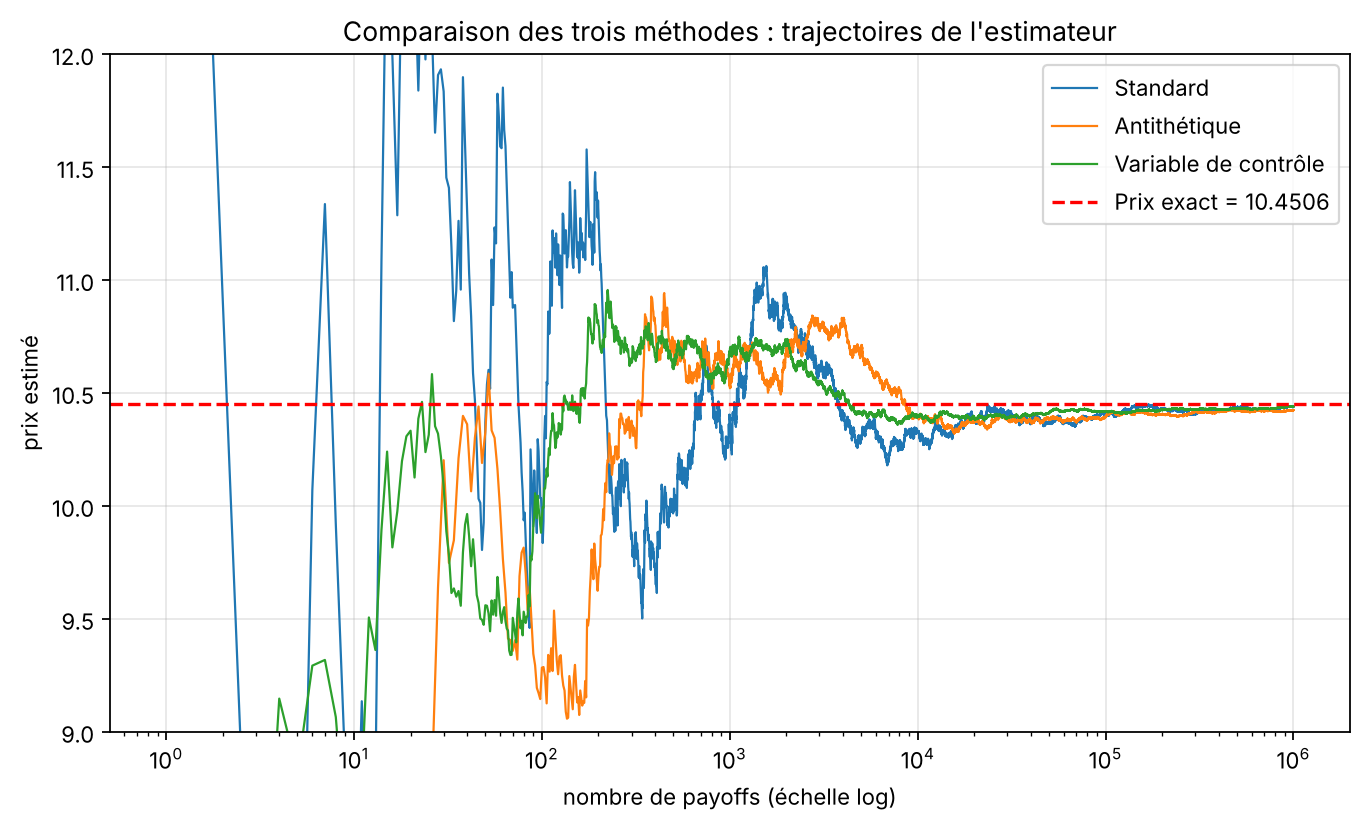
\includegraphics[width=0.82\textwidth]{fig_comparaison_3}
\caption{Moyenne cumulée de chaque méthode en fonction du nombre de payoffs (même budget).}
\label{fig:cmp3}
\end{figure}
Les trois trajectoires convergent vers $\CBS$ ; celle de la variable de contrôle oscille le moins.

\subsection{Prix pour les puissances de 10 : les trois méthodes}
\begin{table}[H]
\centering\small
\begin{tabular}{rcccccc}
\toprule
$N$ & Standard & erreur & Antithétique & erreur & Contrôle & erreur \\
\midrule
10 & 8,3558 & 2,0948 & 4,7035 & 5,7471 & 12,4296 & 1,9790 \\
100 & 7,6188 & 2,8318 & 10,2746 & 0,1760 & 10,9364 & 0,4858 \\
1\,000 & 10,3919 & 0,0587 & 10,4630 & 0,0124 & 10,0182 & 0,4324 \\
10\,000 & 10,2897 & 0,1609 & 10,4057 & 0,0448 & 10,5298 & 0,0793 \\
100\,000 & 10,4781 & 0,0275 & 10,4207 & 0,0299 & 10,4459 & 0,0046 \\
1\,000\,000 & 10,4486 & 0,0020 & 10,4693 & 0,0187 & 10,4516 & 0,0010 \\
\bottomrule
\end{tabular}
\caption{Prix et erreur $|\CBS - \hat C|$ des trois méthodes pour $N = 10^1, \dots, 10^6$.}
\end{table}
Pour $N$ petit, il y a trop peu de tirages et le prix peut être loin de $\CBS$. Quand $N$ grandit, les trois prix s'en rapprochent. Une seule simulation ne suffit pas pour comparer la précision : on répète donc le calcul à $N$ fixé.

\subsection{Stabilité des trois méthodes à $N = 10^6$ fixé}
On refait le calcul $M = 50$ fois avec chaque méthode ($N = 10^6$, nouveaux tirages à chaque fois). L'\textbf{erreur moyenne} est $\frac{1}{50}\sum_{j=1}^{50}|\CBS - \hat C_j|$.
\begin{figure}[H]
\centering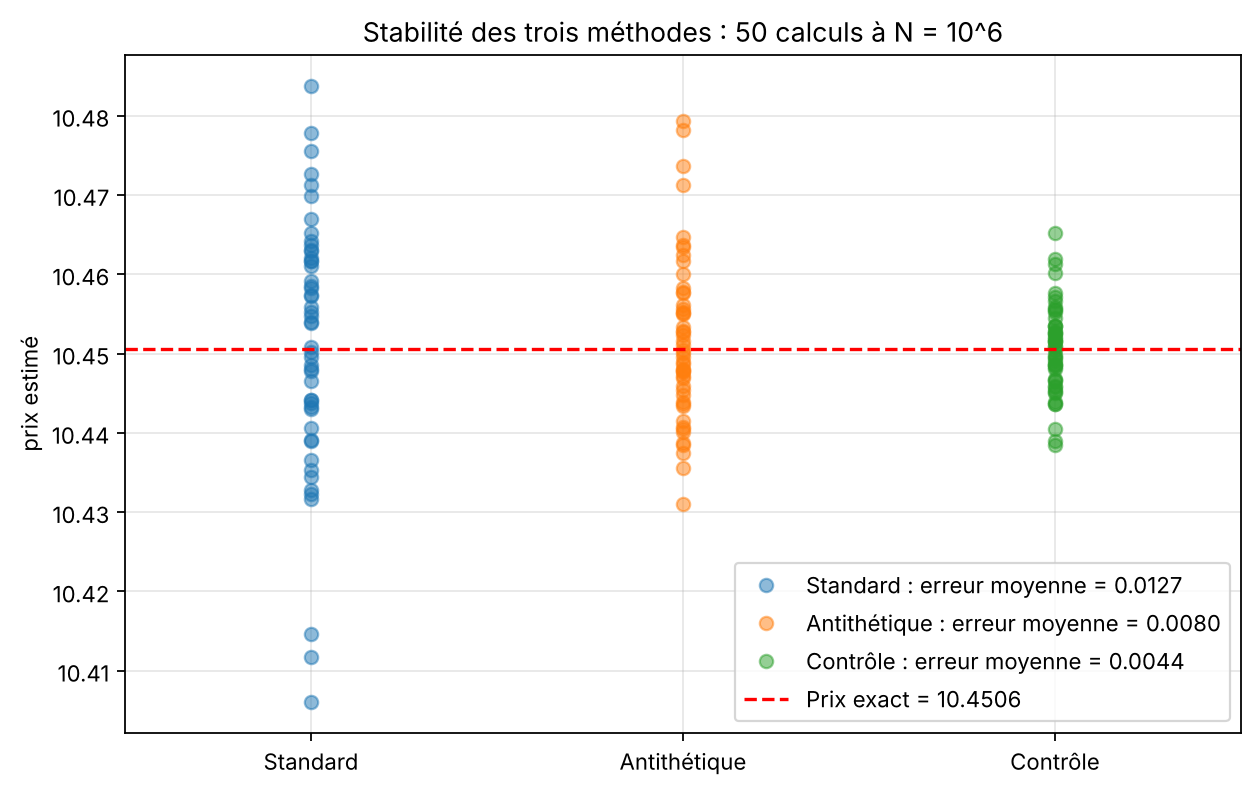
\includegraphics[width=0.78\textwidth]{fig_stabilite_3}
\caption{Les 50 prix de chaque méthode ; la ligne rouge est le prix exact.}
\label{fig:stab}
\end{figure}
\begin{table}[H]
\centering\small
\begin{tabular}{lccc}
\toprule
Méthode & Moyenne des 50 prix & Écart-type & \textbf{Erreur moyenne} \\
\midrule
Standard & 10,4512 & 0,01619 & \textbf{0,01265} \\
Antithétique & 10,4517 & 0,01052 & \textbf{0,00800} \\
Contrôle & 10,4507 & 0,00567 & \textbf{0,00440} \\
\bottomrule
\end{tabular}
\caption{Stabilité à $N = 10^6$ fixé (50 répétitions).}
\end{table}
Les trois colonnes sont centrées sur $\CBS$ (pas de biais). La variable de contrôle est la plus stable : son erreur moyenne est environ 3 fois plus petite que celle du standard. L'écart-type des 50 prix est proche du $SE$ calculé une seule fois, ce qui confirme les intervalles de confiance.

\subsection{La courbe de gain}

\begin{figure}[H]
\centering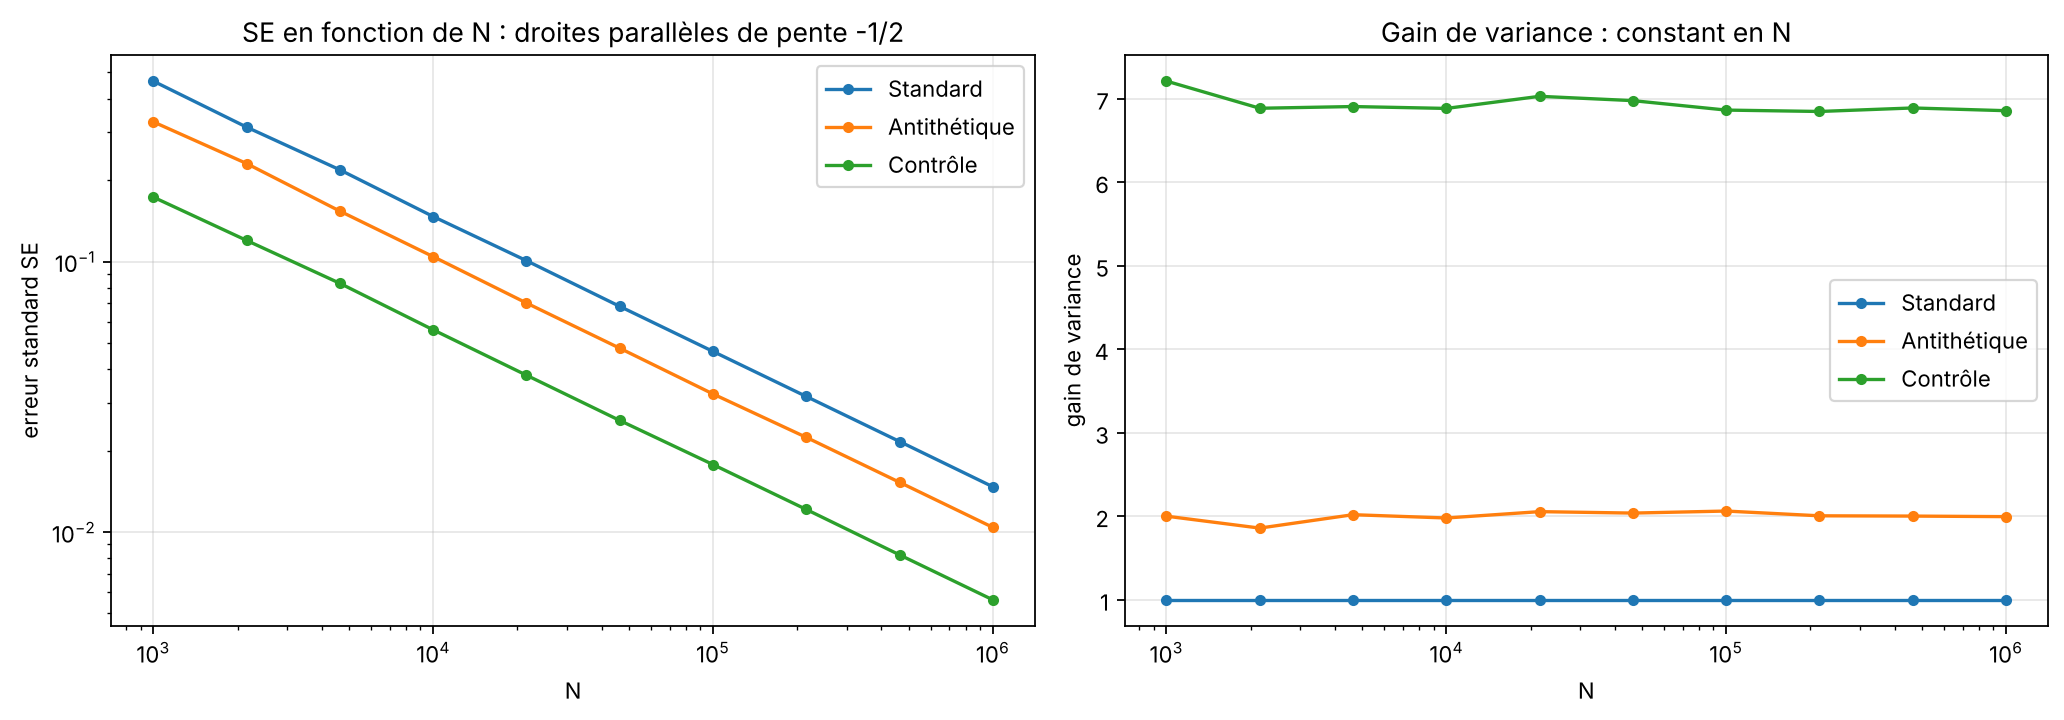
\includegraphics[width=\textwidth]{fig_courbe_gain}
\caption{Gauche : erreur standard des trois méthodes en fonction de $N$ (log-log). Droite : gain de variance en fonction de $N$.}
\label{fig:gain}
\end{figure}

\begin{question}{pourquoi avoir tracé une courbe de gain ?}
Le gain répond à la question pratique : \emph{combien de simulations économise-t-on ?} Un gain de 7 signifie que la méthode atteint avec $N$ simulations la précision que le Monte-Carlo standard atteint avec $7N$. La courbe montre deux choses :
\begin{enumerate}[nosep]
\item \textbf{à gauche}, trois droites \emph{parallèles de pente $-1/2$} : la réduction de variance \emph{ne change pas la vitesse} $1/\sqrt N$, elle \emph{abaisse la droite} d'un facteur $\sqrt{\text{gain}}$ ;
\item \textbf{à droite}, le gain est \emph{constant en $N$} (environ 2 pour l'antithétique, environ 7 pour le contrôle) car il ne dépend que de $\rho$.
\end{enumerate}
\end{question}

\begin{question}{pourquoi l'antithétique est-elle la plus basse ?}
Les deux gains dépendent d'une corrélation, mais pas de la même :
\begin{itemize}[nosep]
\item antithétique : gain $= 1/(1+\rho)$ avec $\rho = \Corr(Y^+,Y^-)\approx-0{,}50$, soit 2. Le payoff convexe empêche $Y^+$ et $Y^-$ de se compenser complètement ;
\item contrôle : gain $= 1/(1-\rho_{XY}^2)$ avec $\rho_{XY} = \Corr(Y,S_T)\approx0{,}92$, soit environ 7. Cette fonction augmente très vite quand $\rho$ s'approche de 1.
\end{itemize}
L'antithétique utilise seulement la \emph{symétrie} de la loi de $Z$ ; la variable de contrôle utilise une \emph{information en plus}, l'espérance exacte de $S_T$. Il est donc normal qu'elle fasse mieux.
\end{question}
